% ------------------------------------------------------ %
% Unofficial Heilbronn University (HHN) LaTeX Template   %
% By Pascal Graf                                         %
% Last Changed: 30.10.2020                               %
% ------------------------------------------------------ %

% Choose paper size, font size and type of the work:
	% usually "report" for long documentations 
	% otherwise "article" for shorter documents (has no \chapter)
\documentclass[a4paper, 11pt]{report} 
% Language Selection, Quotes
\usepackage[english]{babel}
\usepackage[utf8]{inputenc} % Deutsche Umlaute
  %\usepackage[ansinew]{inputenc}
\usepackage[babel]{csquotes}


% Header and Footer Control
\usepackage{fancyhdr}
\usepackage[left=4cm,right=4cm,top=3cm,bottom=3cm,includeheadfoot]{geometry}

% Mathematical Symbols
\usepackage{amsmath}

% Graphics
\usepackage{graphicx}
\usepackage{here}
%\usepackage{subcaption}

% Hyperlinks
\usepackage[hyphens,spaces,obeyspaces]{url}
\usepackage[colorlinks, urlcolor = blue, linkcolor = black, citecolor = black]{hyperref}

% Color
\usepackage{color}

% Blankpage and Blindtext
\usepackage{blindtext} % Enables you to enter some dummy text in sections not written yet
\usepackage{afterpage} 
\newcommand\blankpage{ % Creates a new command for blank pages without header/footer
    \null
    \thispagestyle{empty}
    \addtocounter{page}{-1}
    \newpage}
    
% Titlepage
\usepackage{titling}

% Chapter Style
\usepackage{titlesec}
\definecolor{gray75}{gray}{0.75}
\newcommand{\hsp}{\hspace{15pt}}
\titleformat{\chapter}[hang]{\Huge\bfseries}{\thechapter\hsp\textcolor{gray75}{\textbar}\hsp}{0px}{\Huge\bfseries}

% Pagination Depth
\setcounter{tocdepth}{3} % Depth of the Table of Contents (e.g. (3) means 1.1.1.1 is the maximum depth)
\setcounter{secnumdepth}{4} % Maximum section depth of numbering in the actual document

% BibliographyStyle
\usepackage[numbers]{natbib}
\bibliographystyle{plainnat} 


% ------------------ Begin of the Header and Footer Design --------------------

\fancypagestyle{title_page} % Title Page Header and Footer
{
   	\fancyhf{} % Clear all fields
   	\renewcommand{\headrulewidth}{0pt}
   
   	\fancyhead[R]{}%
\includegraphics[height=70px]{images/HHNLogo}}  
  	\renewcommand{\footrulewidth}{1pt}
	\fancyfoot[C]{\thepage}
}

\fancypagestyle{text_pages} % Normal text Pages Header and Footer
{   
	\fancyhf{} % Clear all fields
	\renewcommand{\headrulewidth}{1pt}
	\fancyhead[L]{\leftmark}
	\fancyhead[R]{}%\rightmark

    \renewcommand{\footrulewidth}{1pt}
	\fancyfoot[L]{}
	\fancyfoot[C]{\thepage}
	\fancyfoot[R]{}     
}

\fancypagestyle{plain} % First Chapter Pages Header and Footer
{   
	\fancyhf{} % Clear all fields
	\renewcommand{\headrulewidth}{1pt}
  	\fancyhead[L]{Thesis Title \\ Denise Baumann\\ Martin Haag}
  	\fancyhead[R]{Heilbronn University \\ Automotive Systems Engineering\\ Mechatronics and Robotice}
  	
  	\renewcommand{\footrulewidth}{1pt}
  	\fancyfoot[L]{Master Project}
  	\fancyfoot[C]{\thepage}
  	\fancyfoot[R]{Winter Semester 2021/22}     
}

% --- Begin of the Actual Document ---
\begin{document}
\pagenumbering{roman}

% --- Title Page Design ---
\input{chapters/00_TitlePage.tex}
\pagestyle{text_pages}

% --- Abstract ---
%\chapter{Einleitung}
\label{ch:Einleitung}

In Einleitungskapitel werden die Rahmenbedingungen des Projekts erläutert.
In diesem Zuge sollen die Ausgangssituation und das Ziel genauer behandelt werden.
\section{Ausgangssituation}
\label{sect:Ausgangssituation}

Am Zentrum für maschinelles Lernen (ZML) wurde bereits in einer vorangegangenen Arbeit an einem selbst spielenden Airhockeytisch gearbeitet. Dazu wurde bereits ein Airhockeytisch mit der benötigten Hardware ausgestattet. Die Kinematik basiert dabei auf der des Roboters von jjRobots \cite{jjrob}

Das Zentrum für maschinelles Lernen (ZML) mchte einen selbstlernenden und spielenden AirHockeyRoboter entwickeln. Dafr statteten Maschinenbaustudenten einen AirHockeyTisch mit einem Kamerahalter und einem Roboter aus, welcher auf dem Konzept
der Firma jjRobots [1] basiert.
Air-Hockey ist ein hochdynamisches Geschicklichkeitsspiel, bei dem zwei Personen gegeneinander spielen. Hierfür sind die Spieler mit einem Pusher ausgestattet. Ziel des Spiels
ist es, den auf einem Luftfilm gleitenden Puck im gegnerischen Tor zu versenken. Durch
die hohen Geschwindigkeiten, welche sowohl den Puck, als auch die Pusher erreichen, besteht ein immenser Anspruch an die Mechanik, sowie an die informationsverarbeitenden
Systeme des gesamten Roboters.Das Zentrum für maschinelles Lernen (ZML) möchte einen selbstlernenden und spielenden Air-Hockey-Roboter entwickeln. Dafr statteten Maschinenbaustudenten einen AirHockey-Tisch mit einem Kamerahalter und einem Roboter aus, welcher auf dem Konzept
der Firma jjRobots [1] basiert.
Air-Hockey ist ein hochdynamisches Geschicklichkeitsspiel, bei dem zwei Personen gegeneinander spielen. Hierfür sind die Spieler mit einem Pusher ausgestattet. Ziel des Spiels
ist es, den auf einem Luftfilm gleitenden Puck im gegnerischen Tor zu versenken. Durch
die hohen Geschwindigkeiten, welche sowohl den Puck, als auch die Pusher erreichen, besteht ein immenser Anspruch an die Mechanik, sowie an die informationsverarbeitenden
Systeme des gesamten Roboters.





%\cite{sutton2018reinforcement}
\newpage


% --- Table of Contents ---
\tableofcontents
\pagenumbering{arabic}

% --- Introduction ---
\chapter{Einleitung}
\label{ch:Einleitung}


In Einleitungskapitel werden die Rahmenbedingungen des Projekts erläutert.
In diesem Zuge sollen die Ausgangssituation und das Ziel genauer behandelt werden.
\section{Ausgangssituation}
\label{sect:Ausgangssituation}
Airhockey ist ein hochdynamisches Geschicklichkeitsspiel, bei dem zwei Personen gegen einander spielen. Hierfür sind die Spieler mit einem Pusher ausgestattet. Ziel des Spiels
ist es, den auf einem Luftfilm gleitenden Puck im gegnerischen Tor zu versenken. Durch
die hohen Geschwindigkeiten, welche sowohl den Puck, als auch die Pusher erreichen, besteht ein immenser Anspruch an die Mechanik, sowie an die informationsverarbeitenden
Systeme des gesamten Roboters.
Am Zentrum für maschinelles Lernen (ZML) wurde bereits in einer vorangegangenen Arbeit an einem selbst spielenden Airhockeytisch gearbeitet. Dazu wurde bereits ein Airhockeytisch mit der benötigten Hardware ausgestattet. Die Kinematik basiert dabei auf der des Roboters von jjRobots \cite{jjrob}
Das Zentrum für maschinelles Lernen (ZML) möchte einen selbstlernenden und spielenden AirHockeyRoboter entwickeln. Dafür statteten Maschinenbaustudenten einen Airhockeytisch mit einem Kamerahalter und einem Roboter aus, welcher auf dem Konzept
der Firma jjRobots basiert.



\newpage

\chapter{Simulationsumgebung}  
\label{ch:Simulationsumgebung}
Ohne eine angemessene Simulationsumgebung ist das ganze Projekt undenkbar. Nicht nur, dass das Training am realen Demonstrator schon wegen des Zeitaufwandes praktisch nicht möglich ist, auch die Konsistenz der Umgebung ist infrage zu stellen.
Die Integration der vielen Rewards sind mit der Bildverarbeitung auch komplizierter und in einer Simulation zusätzlich präziser.
Da wegen vielen Gründen eine Simulation nötig ist und diese auch einen großen Teil der Arbeit ausgemacht hat, wird im folgenden Kapitel das Programm Unity vorgestellt. Außerdem wird unser Unity Projekt hinsichtlich der Implementierung und der Nutzung vorgestellt.

\section{Auswahl  der Umgebung}
\label{sect:Auswahl  der Umgebung}
Da bereits aus einer vorhergegangenen Arbeit und ein Projekt in Unity vorhanden war, ist die Entscheidung hier sehr schnell gefallen.
Selbst ohne diesen Aspekt ist Unity aber eine gute Wahl. Neben einer Pythonschnittstellte, die für Reinforcemet Learning generell immer nützlich ist, kann Unity auch noch mit einer großen Community und sehr guter Dokumentation punkten. Dadurch ist die Einarbeitungsphase relativ kurz und angenehm. Hinzu kommt noch die Toolbox ML-Agents. Diese stellt bereits Agenten zur Verfügung, bei denen nur noch Hyperparameter gewählt werden müssen. Dies ebnet die Möglichkeit, schnelle und unkompliziert mit dem Training zu beginnen.

\section{Unity}
\label{sect:Unity}
Unity ist eine von Unity Technologies entwickelte Multiplattformentwicklungsumgebung zum Erstellen von Videospielen. Für dieses Projekt ist die Anwendung zwar kein Videospiel im herkömmlichen Sinn, aber die Physikengine ist hierfür trotzdem nützlich. Neben dreidimensionalen Umgebungen bietet Unity auch einen 2D-Modus an, der für unsere Anwendung ausreichend ist. Die Programmiersprache unserer Wahl ist c\#, jedoch ist es auch möglich, in UnityScript und Boo benutzerdefiniertes Verhalten zu programmieren.\\
Für dieses Projekt wurde die Unity Version 2020.1.6f1 genutzt.\\
Die Version des ML-Agents Toolkits, die zum Einsatz kam, lautet 2.1.0-exp.1

\subsection{Kurze Einführung}
\label{subsect:Kurze Einführung}

Die kurze Einführung in Unity soll anhand des Userinterfaces geschehen. Diese Einführung ist keineswegs vollständig und soll auch nur ein grobes Verständnis für Fachfremde ermöglichen. Die Markierungen im Bild \ref{untiy_interface} werden im Folgenden erklärt.

\begin{figure}
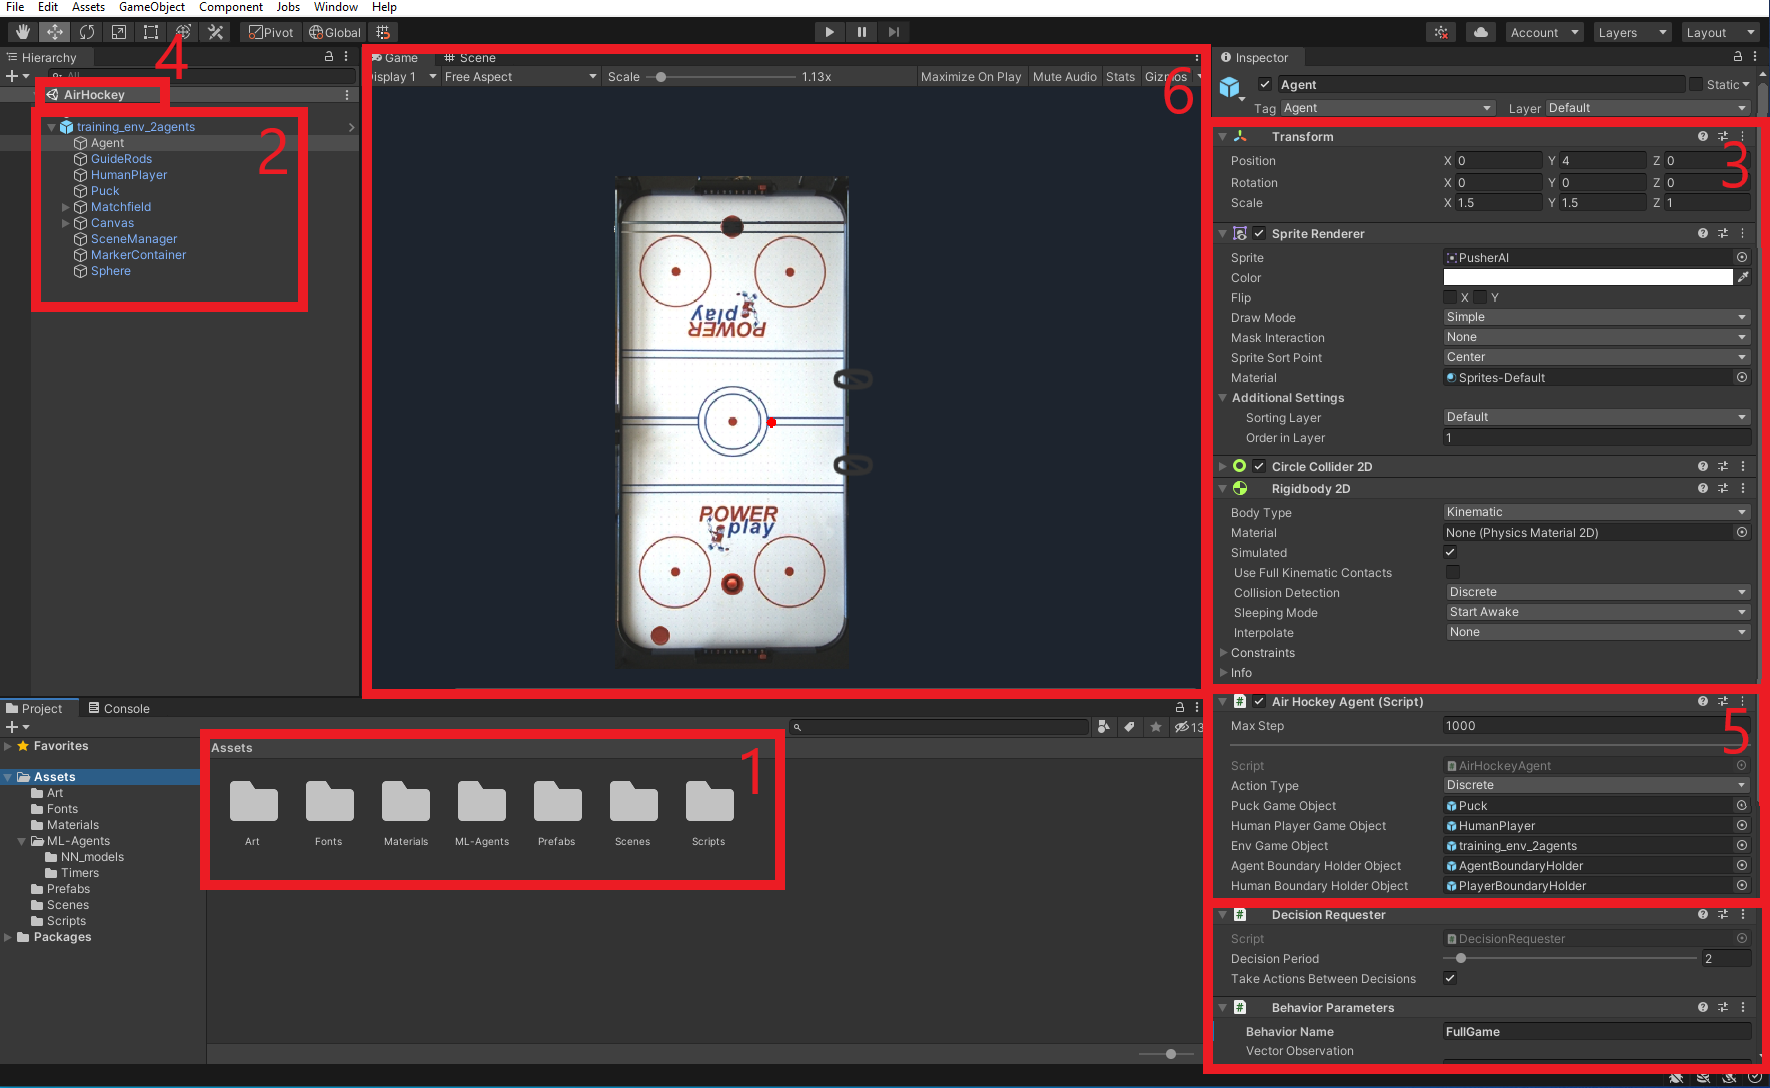
\includegraphics[scale=0.3]{images/unity_interface_marked}
\label{unity_interface_pic}
\caption{Benutzeroberfläche von Unity mit Markierungen}
\end{figure}

\begin{itemize}
\item \underline{Assets (1)} \\
Assets beinhaltet Diverses. Neben Grafiken, vorgefertigten Materialien und Szenen sind hier auch die Skripte zu finden.

\item \underline{GameObjects (2)} \\
GameObjects sind das zentrale Element von Unity. Jedes Objekt, jede Kamera und jede Grafik ist durch ein GameObject definiert. Die Funktionalitäten eines GameObjects werden durch die Components hinzugefügt. Die GameObjects sind in einem Hierarchiebaum in der Scene eingeordnet.

\item \underline{Components (3)} \\
Components geben den GameObjects ihre Funktionalität. Ein GameObject kann mehrere Components haben. Beispiele für Components sind Transform (zuständig für die Position), Collider(zuständig für die Interaktion in der Physiksimulation) und auch Skript.

\item \underline{Scene (4)} \\
Eine Scene (Szene) besteht aus GameObjects. Es ist im Prinzip die Wurzel des Hierarchiebaums. Zur Spieleentwicklung könnten hier unterschiedliche Level als unterschiedliche Scenes interpretiert werden. In unserem Fall sind nur zwei Scenes vorhanden: Eine mit einem Spielfeld zum selbst spielen und testen und eine mit acht Feldern für ein beschleunigtes Training.

\item \underline{Script (5)} :\\
Scripts sind auch Components. Sie bieten die Möglichkeit, das Verhalten selbst zu definieren. Es kann sich in Scripts auf GameObjects bezogen werden. Mit dieser Hilfe können Parameter wie das Material oder die Position geändert werden. Objekte können auch entfernt oder eingefügt werden.

\item \underline{Visualisation (6)} :\\
In diesem Bereich kann sowohl das Bild einer Kamera und  damit die Ansicht im Spiel beobachtet werden als auch eine Darstellung aller GameObjects in der Scene. Objekte können hier auch verschoben oder gedreht werden.
\end{itemize}

\subsection{Airhockey Projekt}
\label{subsect:Airhockey Projekt}

In diesem Unterkapitel werden die einzelnen GameObjects und die wichtigsten Components im Projekt vorgestellt und erklärt. Ziel ist es dabei nicht auf jedes Detail einzugehen, sondern die Arbeit für Folgeprojekte zu erleichtern. Rein optische Aspekte, wie zum Beispiel die Anzeige des Spielstandes, werden nicht betrachtet. Außerdem wird nur auf die Scene mit einem Feld eingegangen, dann die Anpassungen, die zum Kopieren gemacht werden müssen, sind nicht maßgeblich. Die folgenden GameObjects sind auch in der Abbildung \ref{unity_interface_pic} zu finden.\\

\underline{Agent} :

\begin{figure} [h]

\begin{minipage}[t]{0.6\textwidth}
\vspace{0pt}
Der Agent ist eines der zentralen GameObjects. Er hat eine Sprite Renderer Component. Dadurch kann er mit einer .png Datei visualisiert werden. Der Agent ist also ein Objekt, das im Spiel zu sehen ist. Auf der rechten Seite ist die Ansicht, wie sie auch im Projekt zu sehen ist, dargestellt.
\end{minipage}
\hspace{0.1\textwidth}
\begin{minipage}[t]{0.2\textwidth}
\vspace{0pt}

\includegraphics[width=\textwidth]{images/agent_unity}
 \caption{Ansicht des Agenten in Unity}
 \label{unity_agent}
\end{minipage}
\end{figure}

Das Agent GameObject enthält auch eine Circle Colider Component. Mit der Rigidbody Component zusammen wird die Phsyik (Reibung, Bewegung, Kollision) simuliert.\\
Ein weiterer Component des Agent Objekts ist das Script Airhockey Agent. Die Funktion von diesem Script ist die Interaktion mit der ML-Agents Toolbox. Es werden sowohl die anfallenden Rewards entsprechend des Spielverlaufes an das Netzwerk zurückgegeben, als auch die Actions entgegengenommen und damit die Umgebung (Bewegung des Agenten) beeinflusst. Zu Episodenbeginn werden in diesem Script auch die Positionen von Agent und Spieler (Pusher) zurückgesetzt. \\
Des Weiteren beinhaltet das Agent GameObject auch noch eine Decision Requester Component. Mit ihrer Hilfe wird regelmäßig ,entsprechend des Parameters Decision Periode, eine Action vom Netzwerk angefordert. Die Behavior Parameter Componente ist, neben Decision Requester, zur Parametrisierung der Nutzung des ML-Agents Toolkits nötig. Hier kann die Dimension sowohl des Actionspaces als auch die der Observation festgelegt werden. Auch Angaben zur Inferenz können hier gemacht werden. \\


\underline{HumanPlayer} :

\begin{figure} [h]

\begin{minipage}[t]{0.6\textwidth}
\vspace{0pt}
HumanPlayer ist das GameObject des zweiten Spielers. Es hat auch eine Sprite Renderer Component. Die Visualisierung ist rechts zu sehen. Da dieses Objekt auch am Spiel teilnimmt, hat es auch die Components Circle Collider und Rigidbody.
\end{minipage}
\hspace{0.1\textwidth}
\begin{minipage}[t]{0.2\textwidth}
\vspace{0pt}
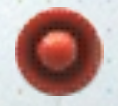
\includegraphics[width=\textwidth]{images/pusher_unity}
 \caption{Ansicht des Pushers in Unity}
 \label{unity_pusher}
\end{minipage}
\end{figure}

HumanPlayer hat auch die Components Decission Requester und Behavior Parameters. Damit wird das Selfplay ermöglicht. In unserer Implementierung wird die Version des Agenten, die den HumanPlayer bewegt nicht trainiert. Das ML-Agents Toolkit wird hier nur zur Inferenz genutzt. \\
Das Objekt enthält auch ein Script. Im Gegensatz zum Airhockey Agents Script werden hier aber keine Rewards zurückgegeben, sondern nur die Observations und die Actions behandelt. Das reicht auch aus, denn dieser Agent soll ja nicht ständig mittrainieren, sondern nur das Selfplay ermöglichen. Wenn er zu schwach wird, wird einfach die stärkere Version vom Agenten übertragen. Im Script ist auch die Option, den HumanPlayer selbst zu steuern, implementiert. Entweder mit der Tastatur oder mit einem Controller kann so der Agent in der Simulation herausgefordert werden. \\

\underline{Puck} :

\begin{figure} [h]

\begin{minipage}[t]{0.6\textwidth}
\vspace{0pt}
Der Puck ist auch ein Objekt, das wie auch der HumanPlayer und der Agent am Spiel teilnimmt. Deshalb hat es auch die Components Circle Collide und Rigidbody.  Die Components, die für das ML-Agents Toolkit nötig sind, werden hier aber nicht verwendet. Trotzdem gibt es auch hier ein c\# Script, das das Verhalten des Pucks bestimmt.
\end{minipage}
\hspace{0.1\textwidth}
\begin{minipage}[t]{0.2\textwidth}
\vspace{0pt}
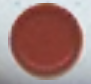
\includegraphics[width=\textwidth]{images/puck_unity}
 \caption{Ansicht des Pucks in Unity}
 \label{unity_puck}
\end{minipage}
\end{figure}
Abhängig vom Spielszenario werden in diesem Script die Startposition und die Startgeschwindigkeit des Pucks festgelegt. Auch der Spielstand wird hier mitgezählt. Die Circle Collider Componente  des Pucks erlaubt es, ein Event bei Kollision mit anderen Objekten auszulösen. Wenn der Spielfeldrand am Tor des Agenten getroffen wird, kann das mithilfe eines GameObjects ohne Renderer erkannt werden. Es kann mit einer Box Collider Componente ein Event ausgelöst werden, das den Spielstand anpasst. Das gleiche System wird auch auf der anderen Seite angewendet. \\

\underline{Matchfield} :

\begin{figure} [h]

\begin{minipage}[t]{0.6\textwidth}
\vspace{0pt}
Das GameObject Matchfield hat selbst nur eine Sprite Renderer Component, die ein Bild des Airhockeytisches zeigt. Jedoch sind diesem Objekt hierarchisch Weitere untergeordnet. Diese untergeordneten Objekte sind aber alle ohne Renderer Component und deshalb in der Spielansicht unsichtbar. Sie sind nur wegen ihrer Position interessant. Sie dienen dazu, das Spielfeld in Zonen einzuteilen. Die zulässigen Positionen von Agent, HumanPlayer und Puck werden damit auf das Spielfeld oder die jeweilige Hälfte limitiert. Die GameObjects, die zum Torezählen genutzt werden, sind auch Childobjects (hierarchisch untergeordnete Objekte) des Matchfields.
\end{minipage}
\hspace{0.1\textwidth}
\begin{minipage}[t]{0.2\textwidth}
\vspace{0pt}
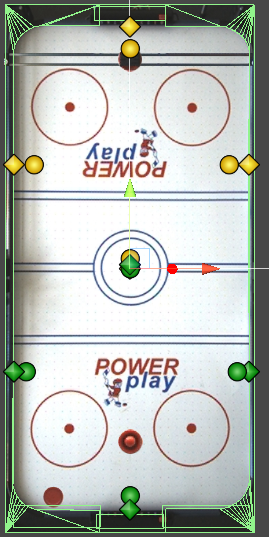
\includegraphics[width=\textwidth]{images/matchfield}
 \caption{Spielfeldbegrenzungen in Unity}
 \label{unity_matchfield}
\end{minipage}
\end{figure}
Das Matchfield hat kein Script, es wird sich nur von anderen Scripts auf die GameObjects von Matchfield bezogen. Die Transform Component, die die Position eines Objects angibt, wird dabei ausgelesen. Mit vier Objekten lässt sich damit ein rechteckiger Bereich festlegen. \\

\underline{training\_env\_2agents} :\\
Diesem Objekt sind, abgesehen von der Kamera, alle anderen GameObjects untergeordnet. Es dient als Container für das ganze Spiel. Das Objekt dient hauptsächlich zwei Zwecken:
\begin{itemize}
\item Das ganze Spielfeld kann einfacher kopiert und verschoben werden. Die Positionen der Childobjects bleiben beim Verschieben des übergeordneten Objekts relativ zu diesem unverändert. Felder könne dadurch schnell über und nebeneinander kopiert werden.
\item Das envScript ist in diesem GameObject ein Component. In diesem Script werden alle Rewards festgelegt. Auch der Spielmodus wird hier ausgewählt. Näheres zu den Rewards und den Spielmodi wir im Kapitel \ref{subsect:Airhockey Projekt} erläutert.
\end{itemize}

% --- Bibliography ---
\bibliography{bibfile} 
\bibliographystyle{ieeetr}


\end{document}